\documentclass{article}
\usepackage{fancyhdr}
\usepackage{ctex}
\usepackage{listings}
\usepackage[a4paper, body={18cm,22cm}]{geometry}
\usepackage{amsmath,amssymb,amstext,wasysym,enumerate,graphicx}
\usepackage{float,abstract,booktabs,indentfirst,amsmath}
\usepackage{multirow}
\usepackage{enumitem}
\usepackage{listings}
\usepackage{xcolor}
\usepackage{tabularx}
\usepackage[most]{tcolorbox}
\usepackage{accsupp}
\usepackage[bottom]{footmisc}
\usepackage{subcaption}
% \usepackage[backend=biber,style=numeric]{biblatex}
\usepackage[xetex]{hyperref}
\usetikzlibrary{arrows.meta}
\newcommand\emptyaccsupp[1]{\BeginAccSupp{ActualText={}}#1\EndAccSupp{}}
\setlength{\parindent}{2em}
\renewcommand\arraystretch{1.4}
\setmonofont{Fira Code}
\setCJKmonofont{黑体}
% \setmainfont{Times New Roman}
\hypersetup{CJKbookmarks=true,colorlinks=true,citecolor=blue,%
            linkcolor=blue,urlcolor=blue,bookmarksnumbered=true,%
            bookmarksopen=true,breaklinks=true}
\lstset{
    % language = C,
    xleftmargin = 3em,xrightmargin = 3em, aboveskip = 1em,
	backgroundcolor = \color{white}, % 背景色
	basicstyle = \small\ttfamily, % 基本样式 + 小号字体
	rulesepcolor= \color{gray}, % 代码块边框颜色
	breaklines = true, % 代码过长则换行
	numbers = left, % 行号在左侧显示
	numberstyle = \small\emptyaccsupp, % 行号字体
    numbersep = -14pt, 
    keywordstyle=\color{purple}\bfseries, % 关键字颜色
    commentstyle =\color{red!50!green!50!blue!60}, % 注释颜色
    stringstyle = \color{red}, % 字符串颜色
    morekeywords={ASSERT, int64_t, uint32_t},
	frame = single, 
	showspaces = false, % 不显示空格
    showstringspaces = false,
	columns = fixed, % 字间距固定
    literate=
        {^-}{{{\color{black}\textbf{\color{red}-}}\colorbox{red!30}{\phantom{XX}}}}{1}
        {^+}{{{\color{black}\textbf{\color{green}+}}\colorbox{green!30}{\phantom{XX}}}}{1},
}

\raggedbottom

\title{\heiti\textbf{Kea 使用报告}}
\author{第七组}
\date{}

\begin{document}
\maketitle

\section{工具简介}

Kea 是一个基于性质的移动应用软件自动化功能测试工具,它将自动化UI遍历与基于性质的测试结合,从而在更好地构建测试预言的同时扩大测试输入空间。

Kea设计了一种面向移动应用的性质描述语言,从而允许用户通过描述前置条件、交互场景和后置条件来定义性质,构建测试预言。同时,Kea还提供了三种页面探索策略:随机遍历、基于主路径遍历、大模型引导的路径遍历,从而自动生成事件序列来达到应用更深层的状态,有效覆盖移动应用事件探索空间。

\section{使用环境}

\begin{itemize}[noitemsep]
    \item 操作系统:Windows 11 家庭中文版 26100.3323
    \item CPU: 11th Gen Intel(R) Core(TM) i7-11800H @ 2.30GHz
    \item Python版本:3.13.2
    \item Kea版本:2.0.4
    \item Android 模拟器:Pixel\_9\_API\_35
\end{itemize}

\section{安装}

Kea 是一个 Python 库,
使用 pip 包的形式发布。

首先需要克隆仓库:

\begin{lstlisting}[language=bash]
    git clone https://github.com/ecnusse/Kea.git
\end{lstlisting}

接着可以通过以下命令安装:

\begin{lstlisting}[language=bash]
    pip install -e .
\end{lstlisting}

安装完成后,就可以在命令行中使用 \texttt{kea} 命令。

\section{Quick Start}

Kea 的文档中提供了一个简单的例子,用于展示 Kea 的基本功能。

\begin{lstlisting}[language=bash]
    kea -f example/example_property.py -a example/omninotes.apk
\end{lstlisting}

在这个例子中,我们使用了一个名为 \texttt{example\_property.py} 的性质文件,来测试 \texttt{omninotes.apk} 中一项基本的性质——旋转屏幕后,搜索框不应该被清空。


\begin{lstlisting}[language=python]
    from kea import *


    class Test(KeaTest): 

        @initializer()
        def pass_welcome_pages(self):
            if d(text="Allow").exists():
                d(text="Allow").click()
            for _ in range(5):
                d(resourceId="it.feio.android.omninotes.alpha:id/next").click()
            d(resourceId="it.feio.android.omninotes.alpha:id/done").click()
    
        @precondition(lambda self: d(resourceId="it.feio.android.omninotes.alpha:id/search_src_text").exists())
        @rule()
        def search_bar_should_exist_after_rotation(self):
            d.rotate('l')
            d.rotate('n')
            assert d(resourceId="it.feio.android.omninotes.alpha:id/search_src_text").exists()
\end{lstlisting}

\texttt{example\_property.py} 如上所示。在使用 Kea 时,我们需要继承 \texttt{KeaTest} 类,并使用库中提供的装饰器来定义性质。

\texttt{@initializer} 装饰器用于定义初始化函数,从而在测试开始前执行一些操作,帮助我们跳过应用程序的欢迎页面或引导等。\texttt{@precondition} 装饰器用于定义前置条件,即在测试性质之前需要满足的条件。\texttt{@rule} 装饰器用于标记这个函数是一个性质。在这个函数中,我们可以进行一些交互操作,并使用 \texttt{assert} 语句来判断性质是否成立。

启动安卓模拟器后,运行上面的命令进行测试。

等待运行结束或者按下 \texttt{Ctrl + C} 提前终止测试,在 \texttt{output} 文件夹中可以查看Kea生成的测试报告。

如图 \ref{fig:1} 展示的测试报告所示,我们可以看到在整个测试过程中每一步的操作和截图。在持续了3607秒的测试中,共发现了11个bug,共出现了21次符合前置条件的情况,其中有11次进行了测试,均没有通过。这足以说明此应用程序在此性质上存在缺陷。

\begin{figure}[H]
\centering
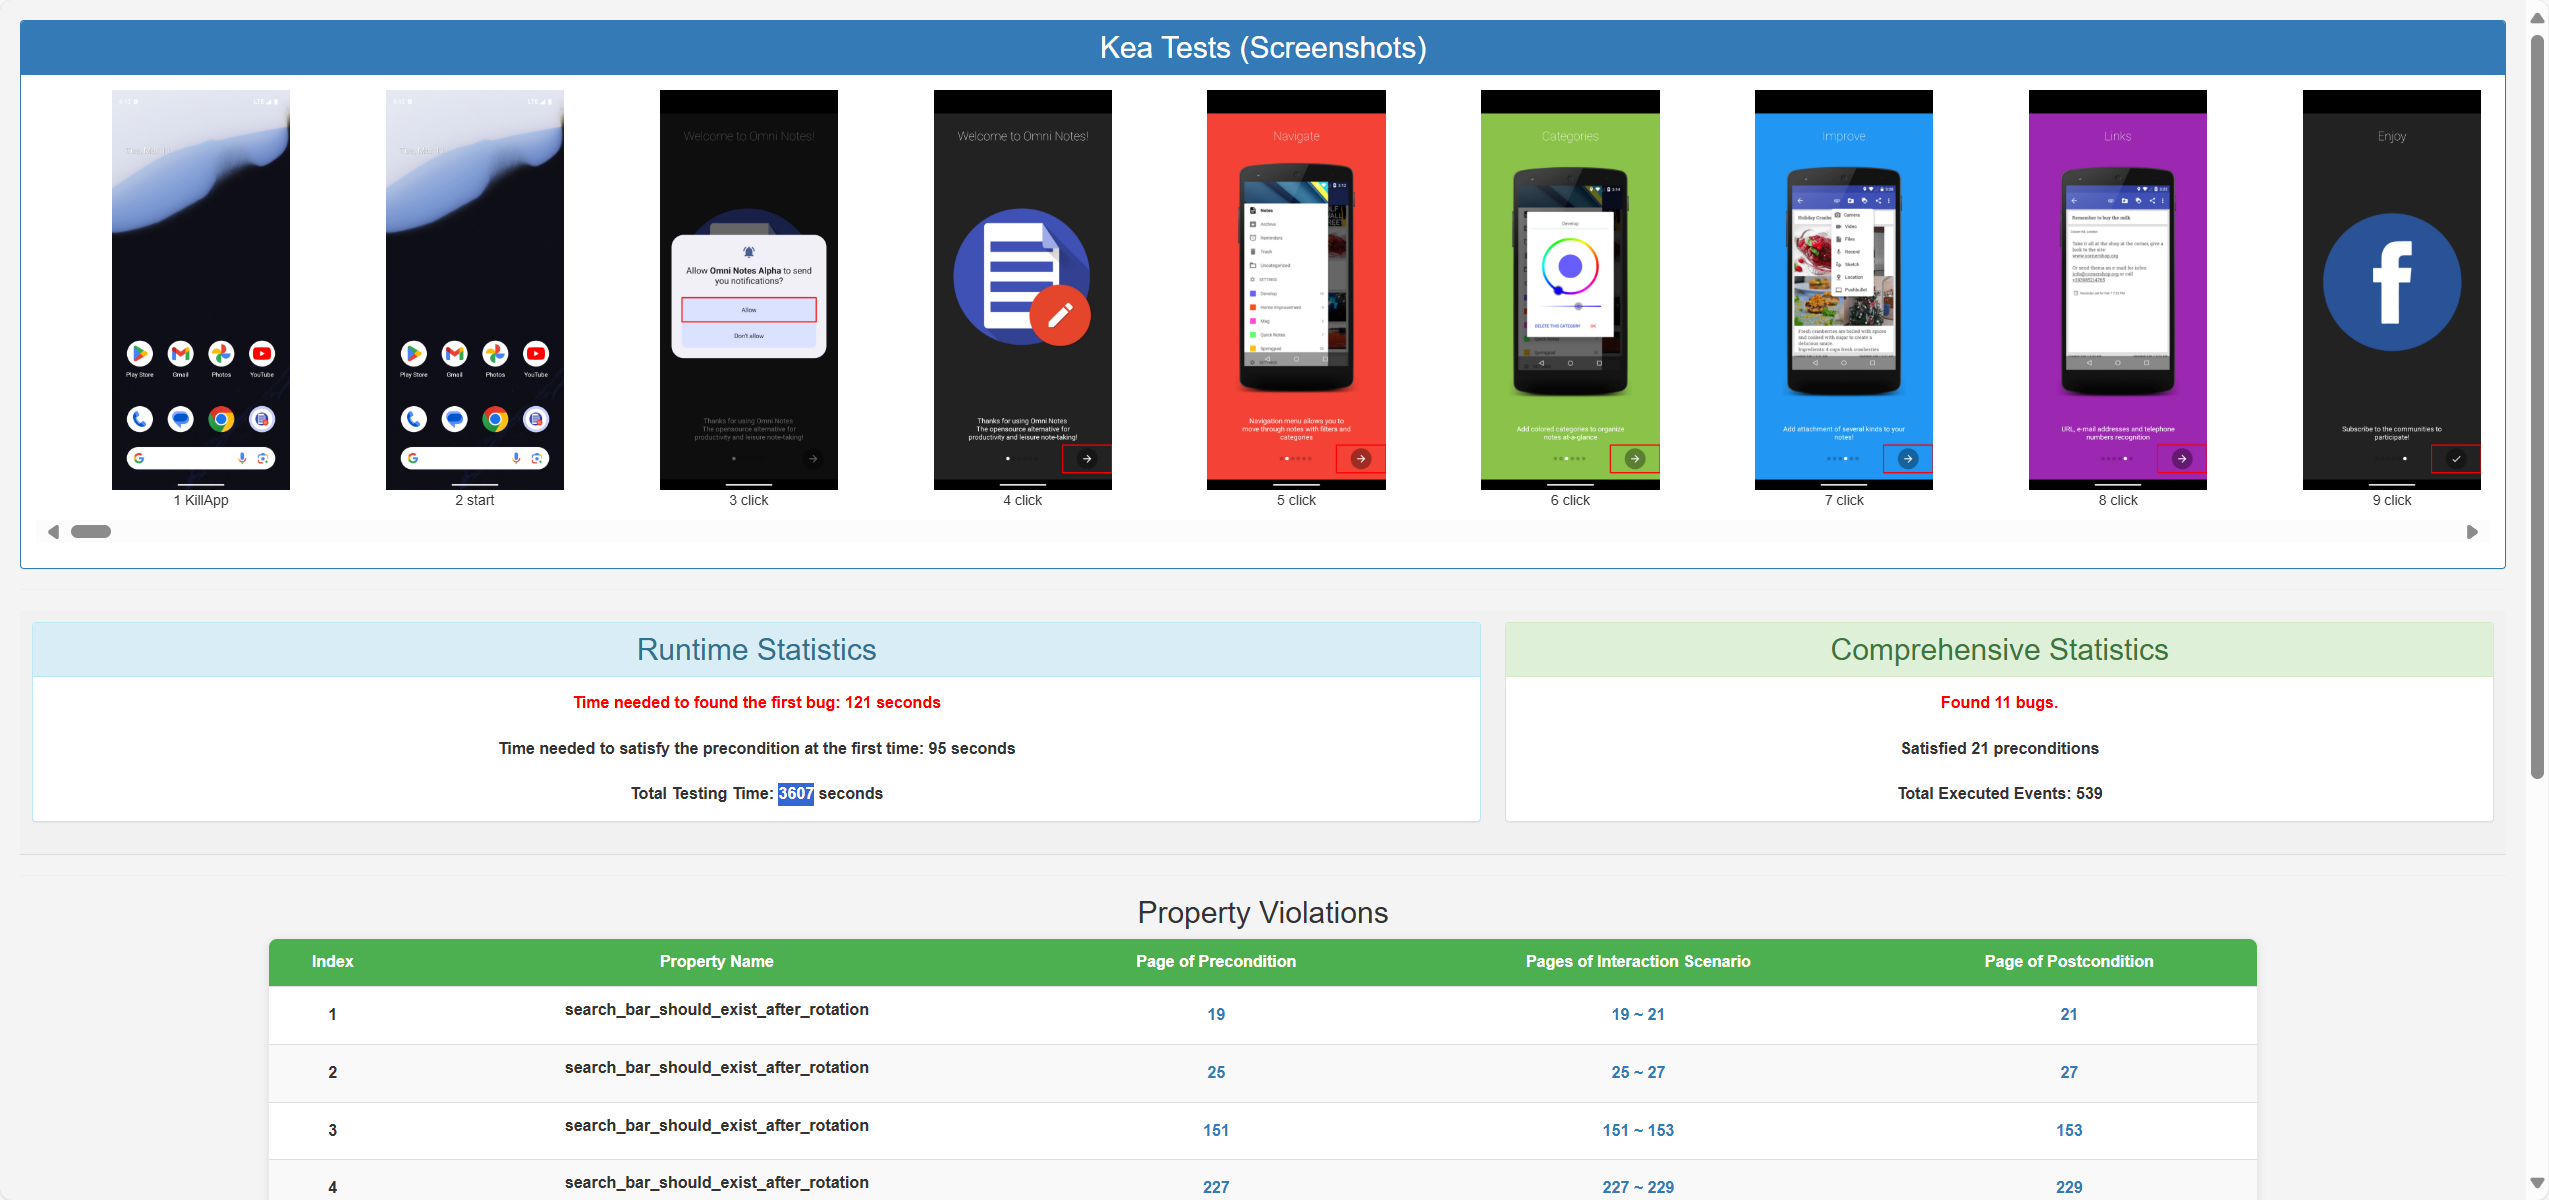
\includegraphics[width=\textwidth]{img/1.png}
\caption{Kea 测试报告}
\label{fig:1}
\end{figure}

\section{进一步使用}

\subsection{主路径引导策略}

除了随机探索的路径遍历策略外,Kea还提供了基于主路径的路径遍历策略。在这种策略下,Kea会根据用户提供的主路径生成事件序列,并在主路径附近进行探索。

\begin{lstlisting}[language=python]
    @mainPath()
    def test_main(self):
        d(resourceId="it.feio.android.omninotes.alpha:id/fab_expand_menu_button").long_click()
        d(resourceId="it.feio.android.omninotes.alpha:id/detail_content").click()
        d(resourceId="it.feio.android.omninotes.alpha:id/detail_content").set_text("read a book #Tag1")
        d(description="drawer open").click()
        d(resourceId="it.feio.android.omninotes.alpha:id/note_content").click()
\end{lstlisting}

如上所示的代码定义了一个主路径,其中包含了一系列的交互操作。Kea可以沿主路径进行探索,并让主路径指导探索。

相比于随机探索,基于主路径的探索策略更容易找到符合前置条件的状态,从而更容易检查性质是否成立,但也不可避免地降低随机性。

\subsection{大模型引导策略}

在修复了一些bug后,我们还尝试了现有的大模型引导策略。该策略在随机探索的基础上,引入了一个大预言模型,用于陷入UI陷阱时指导探索从UI陷阱中逃离。

在命令行启动Kea时,通过 \texttt{-p llm} 参数来启用大模型引导策略。

但在我们的测试中,我们发现,在逃离UI陷阱、提高测试效率上,当前大模型引导策略并不能提供有效的帮助,仍有较大提升空间。

\section{复现示例}

Kea的文档中记载了使用此工具发现的一些开源软件的bug,我们尝试对其中一部分进行了复现,下面是其中一次复现的简要记述:

\begin{itemize}[noitemsep]
    \item 软件名称:amaze
    \item 软件版本:3.10
    \item Bug:当点击历史记录中的文件夹时,FAB按钮没有正确呈现(\url{https://github.com/TeamAmaze/AmazeFileManager/issues/4130})
\end{itemize}

我们定义了如下性质文件:

\begin{lstlisting}[language=python]
    from kea import *

    class Test(KeaTest):
    
        @initializer()
        def set_up(self):
            if d(text="Allow").exists():
                d(text="Allow").click()
            if d(text="GRANT").exists():
                d(text="GRANT").click()
    
        @precondition(lambda _: d(resourceId="com.amaze.filemanager:id/fullpath").exists() and '/' in d(resourceId="com.amaze.filemanager:id/fullpath").info['text'] and not d(resourceId="com.amaze.filemanager:id/check_icon").exists())
        @rule()
        def FAB_should_exist_in_folder(self):
            assert d(resourceId="com.amaze.filemanager:id/sd_main_fab").exists()
            
\end{lstlisting}

该性质文件中定义了一个名为 \texttt{FAB\_should\_exist\_in\_folder} 的性质,用于测试在``文件夹''视图中是否存在FAB按钮。其中,前置条件是当前视图为``文件夹''视图,且当前路径中包含``/'',且当前视图中不存在``check\_icon'',即当前视图不是选择模式。

结果如图 \ref{fig:2} 所示,我们发现了这个bug,即在``文件夹''视图中,FAB按钮没有正确呈现。

\begin{figure}[H]
\centering
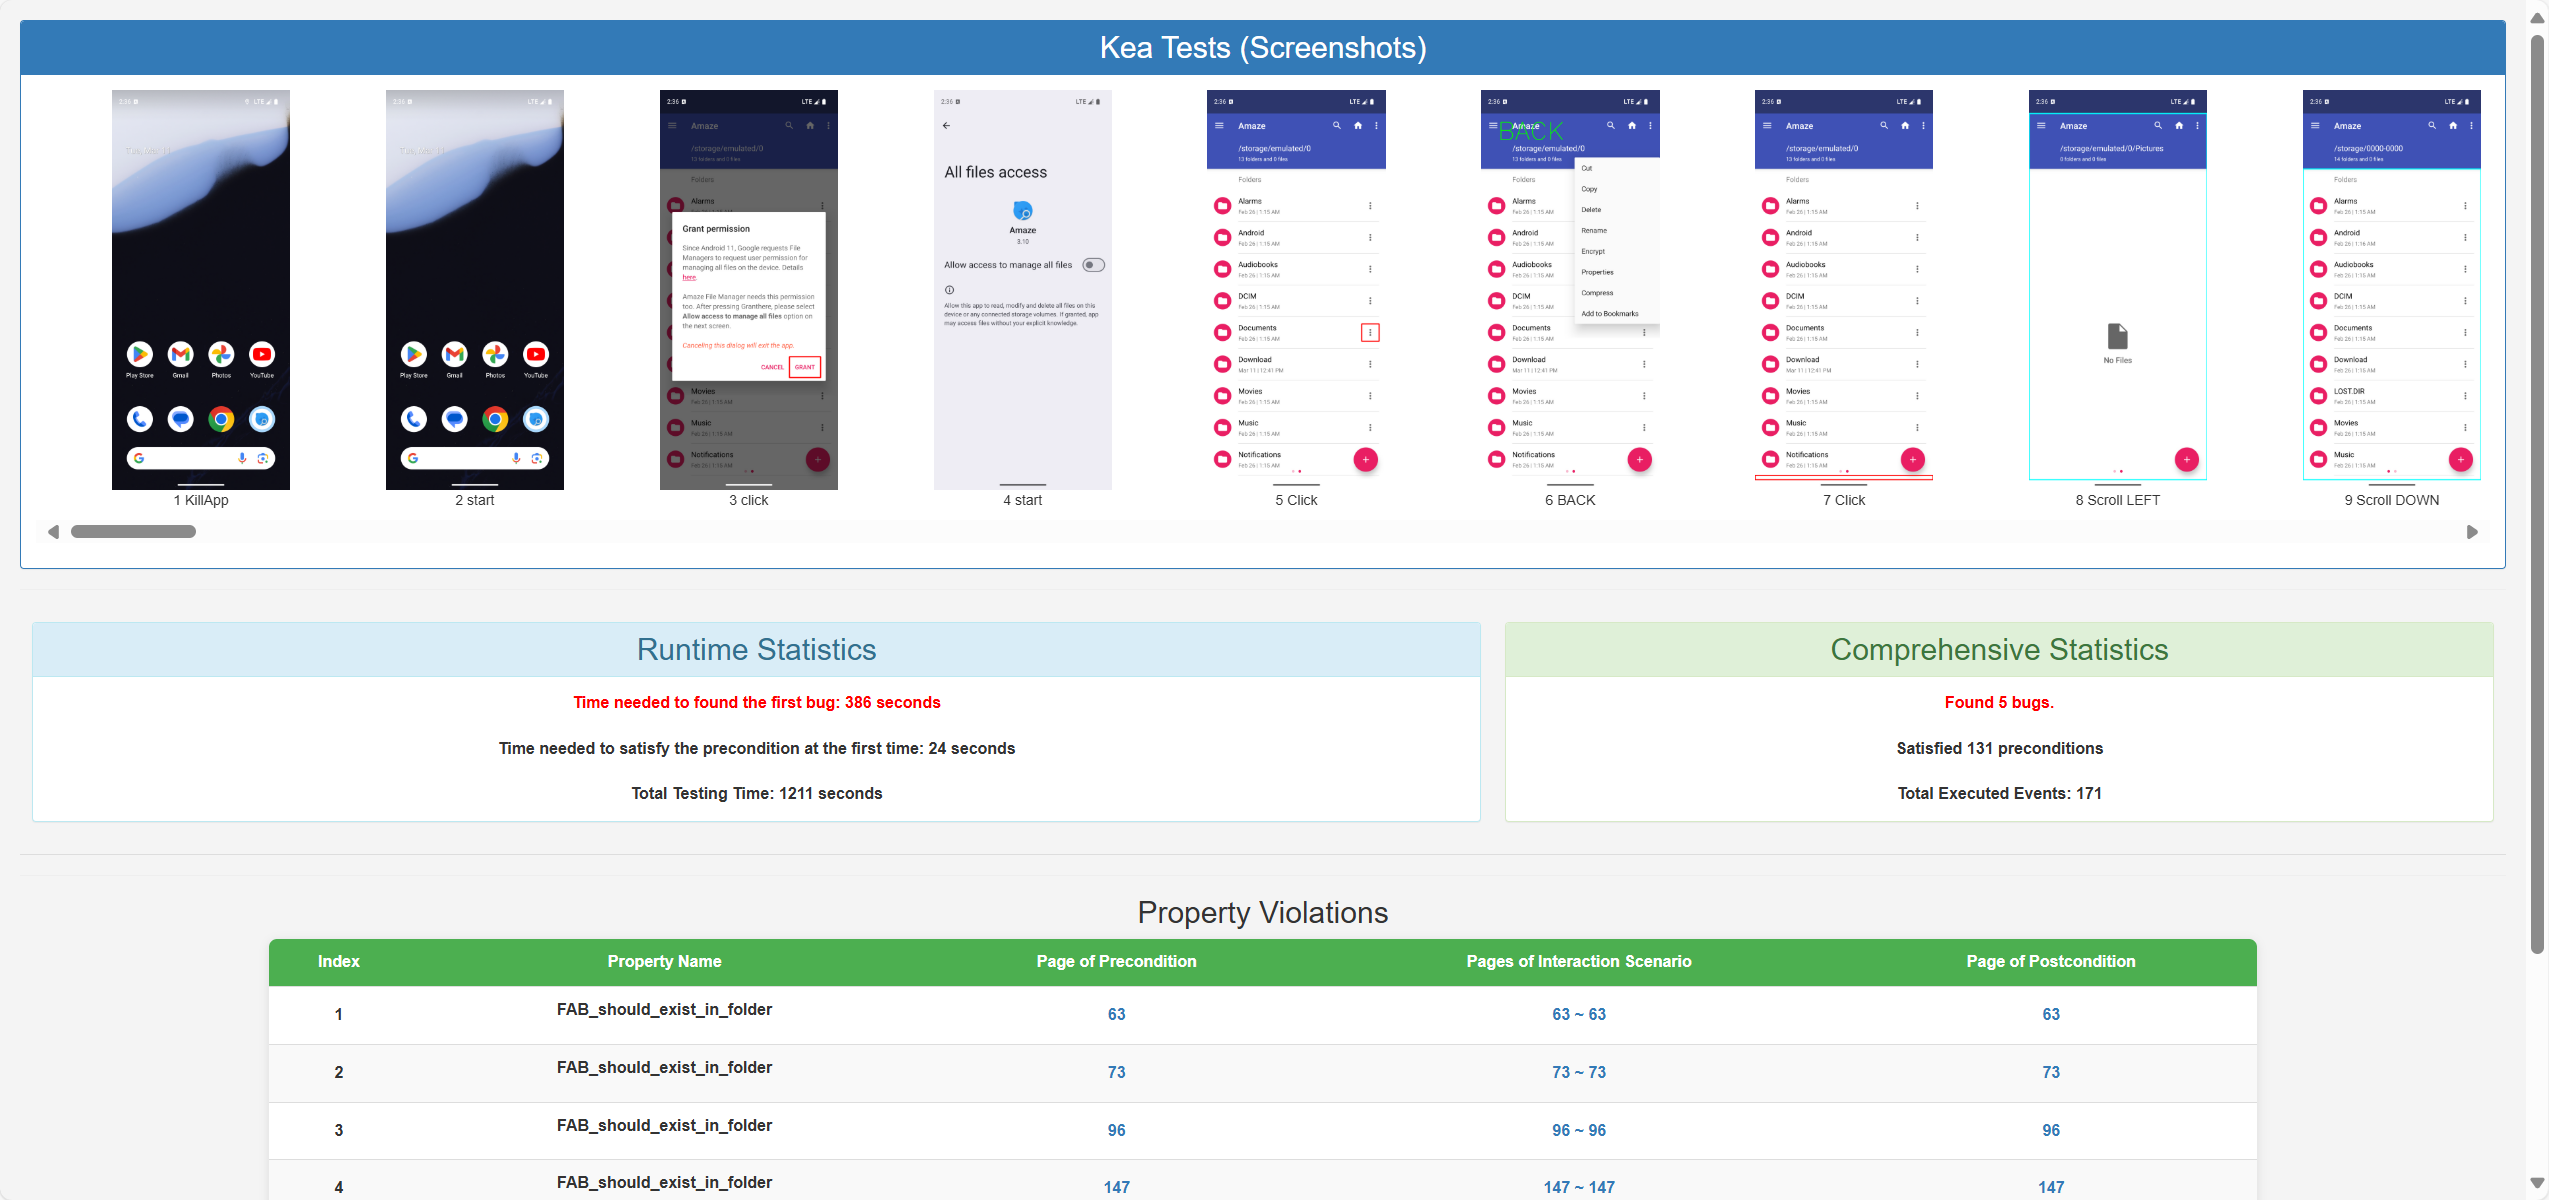
\includegraphics[width=\textwidth]{img/2.png}
\caption{Kea 测试报告}
\label{fig:2}
\end{figure}


\section{发现的BUG}

在使用Kea的过程中,我们也发现了一些bug:

\begin{enumerate}
    \item (已被修复)\texttt{setup.py} 文件中的 \texttt{install\_requires} 字段中的依赖项缺少了包 \texttt{rtree},导致在运行时出现错误。
    \item (部分修复)Kea 关于性质定义的部分文档过时,导致如果按照文档中的方法定义性质会出现错误。见 \url{https://github.com/ecnusse/Kea/issues/35}(已修复) 及 \url{https://github.com/ecnusse/Kea/issues/40}(未修复)。
    \item (未修复,第三方软件bug)在Windows下测试鸿蒙系统模拟器时会出现错误。见 \url{https://github.com/ecnusse/Kea/issues/36} 和 \url{https://github.com/ecnusse/Kea/issues/42}。
    \item (未修复)在使用Kea进行测试时,如果安卓系统通知栏被拉下,Kea会无法正常工作。见 \url{https://github.com/ecnusse/Kea/issues/44}。
    \item (已修复)代码中曾经被上传的API key仍在历史记录中,可能会被其他人使用。见 \url{https://github.com/ecnusse/Kea/issues/41}。
\end{enumerate}

此外,我们还发现了一些与大模型引导策略相关的bug:

\begin{enumerate}
    \item \texttt{LLMPolicy} 类初始化时,未将 \texttt{output\_dir}参数传递给父类,导致启动时出现错误。
    
    缺陷位置:\texttt{input\_policy.py} 第 735 行

    修复方式:

    \begin{lstlisting}[language=bash,numbers=none]
^-   super(LLMPolicy, self).__init__(device, app, kea)
^+   super(LLMPolicy, self).__init__(device, app, kea, output_dir=output_dir)
    \end{lstlisting}

    \item 相似度比较函数存在错误,导致无法正确计算两个状态之间的相似度。
    
    缺陷位置:\texttt{input\_policy.py} 第 770\textasciitilde 800行
    
    修复方式:

    \begin{lstlisting}[language=bash,numbers=none]
    if self.device.is_harmonyos == False and hasattr(self.device, "u2"):
        self.device.u2.set_fastinput_ime(True)

    self.logger.info("Exploration action count: %d" % self.event_count)

^-  if self.to_state is not None:
^-      self.from_state = self.to_state
^-  else:
^-      self.from_state = self.device.get_current_state()

    if self.event_count == 0:
        # If the application is running, close the application.
        event = KillAppEvent(app=self.app)
    elif self.event_count == 1:
        event = IntentEvent(self.app.get_start_intent())
    else:
        if input_manager.sim_calculator.detected_ui_tarpit(input_manager):
            # If detected a ui tarpit
            if input_manager.sim_calculator.sim_count > MAX_NUM_QUERY_LLM:
                # If query LLM too much
                self.logger.info(f"query too much. go back!")
                event = KeyEvent(name="BACK")
                self.clear_action_history()
                input_manager.sim_calculator.sim_count = 0
            else:
                # stop random policy, start query LLM
                event = self.generate_llm_event()
        else:
            event = self.generate_event()

^+  self.from_state = self.device.get_current_state()
    \end{lstlisting}
\end{enumerate}

\end{document}